\documentclass{sig-alternate-05-2015}
\usepackage{float}
\usepackage{hyperref}


\begin{document}
% Copyright
%\setcopyright{acmcopyright}
% DOI
\doi{000000}

% ISBN
\isbn{000000}

\title{Access to Big Data in Bioinformatics}
% \subtitle{[Extended Abstract]}

\numberofauthors{1}
\author{
\alignauthor
Andrew van Rooyen\\
       \affaddr{University of Cape Town}\\
}

\date{30 August 2015}

\toappear{
	This paper and associated code is available at \url{https://github.com/wraithy/bigbinf}\\
	The OpenSSH-Portable installation used for HPN-SSH was compiled frm \url{https://github.com/rapier1/openssh-portable}\\
	The large hg38.fa.align.gz dataset used is available at \url{http://hgdownload.cse.ucsc.edu/goldenPath/hg38/bigZips/}\\
	For more information, please see \url{people.cs.uct.ac.za/~vryand003}
}

\maketitle
\begin{abstract}
	TODO
\end{abstract}
% \keywords{Big Data; BioInformatics; Clouds}


\section{Introduction}
Next generation sequencing has resulted in a massive increase in the size of bioinformatics datasets, which can be tens of gigabytes in size~\cite{deorowicz2011compression}. Sequencing technologies like SOLiD provide much higher data output at a cheaper cost~\cite{shendure2008next}, which creates challenges in data storage, transfer and access. In fact, the cost of storing a byte has been higher than sequencing a base pair since before 2010~\cite{baker2010next}.

\subsection{Data storage}
Generally, sequence data is stored in a data warehouse. Storing this information for long periods of time requires the data to be structured efficiently in order to save space, and to allow it to be transferred efficiently.

There are a plethora of sequence file formats whose efficiency depends on the kind of data stored. Two of the most popular are FASTQ, which stores aggregated reads along with the quality of each DNA base pair~\cite{cock2010sanger}, and BAM, the binary, compressed version of the Sequence Alignment Map (SAM) format~\cite{SAMspec}.

\subsection{Data transfer}
Researchers often require access to the data warehouses to transfer the sequences they need. Luckily, these locations are often connected by massive data pipes like National Research and Education Networks (NRENs). Unfortunately, standard protocols like FTP and SSH were not designed for use on high-throughput networks, and alternate protocols must be used to avoid bottlenecks.

Some proprietary transfer protocols are widely used in practice - for example, the \textit{fasp} protocol by the US based company AsperaSoft. Based on UDP, the protocol eliminates the latency issues seen with TCP, and provides transfer bandwidth of up to 10 gigabits per second~\cite{beloslyudtsev2014aspera}.

\subsection{Alternate models}
There have been some attempts to avoid transferring data. This means processing data remotely, and there has been an explorative push towards cloud solutions from Amazon, Google etc~\cite{baker2010next}. Unfortunately, even though these cloud data centres have plenty of cheap storage, this does not remove the transfer bottleneck as researchers must still upload their raw data to the cloud data centres every time they run a new experiment. Some researchers have even resorted to mailing hard drives~\cite{baker2010next}.

There are also security, privacy and ethical concerns with outsourcing this processing power to other companies, as sequenced DNA data is often highly sensitive information~\cite{marx2013biology}.

\subsection{Investigation}
In this work, we compare the following file transfer protocols to determine which is best for transferring bioinformatics data on an educational network: GridFTP, FTP, HPN-SSH and SSH.
These are the most popular protocols for file transfer in the field, perhaps with the exception of AsperaSoft's \textit{fasp} which is non-free. 

In order to test the protocols in a relevant environment, the tests will be run between the University of Cape Town (UCT) and the University of the Western Cape (UWC). Both universities are connected to the South African National Research Network \cite{sanren} which runs at 10Gbps.

\section{Methods}
\subsection{Protocols}
The OpenSSH~\cite{openssh} implementations of FTP (sftp) and SSH (scp) will be tested. High Performance SSH (HPN-SSH) is a set of patches to OpenSSH which removes bottlenecks~\cite{rapier2008high}. The scp binary from a patched, portable version of OpenSSH will be tested for HPN. This will be installed alongside the original so that both binaries are available.

The `lite' version of GridFTP~\cite{allcock2005globus} will be used. This means that authentication is done via ssh as opposed a previously-configured certificate authority. This makes no difference to the file transfer itself, but it prevents unnecessary configuration of the testbed which can be quite complex in the case of `full' GridFTP~\cite{gridftplite}.

Once the ideal protocol has been decided on, it will be made available as an endpoint to the microcloud system, so that users can retrieve their results in an optimal way.

\subsection{Approach}
Transfers using each of the 4 protocols will be run while the network traffic is logged.

\begin{figure}[H]
	\centering
	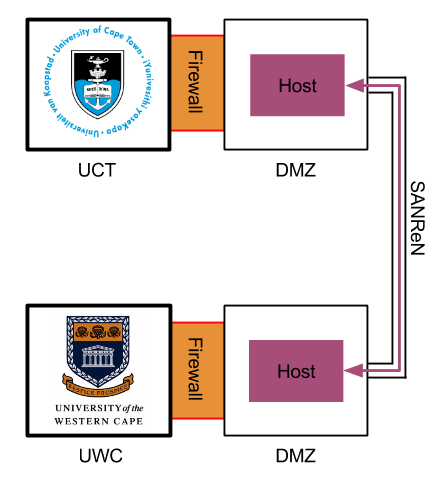
\includegraphics[width=0.4\textwidth]{img/route.png}
	\caption{The hosts in their environment.
	         \label{fig:route}}
\end{figure}

The hosts will be virtual machines running at the South African National Bioinformatics Institute (UWC) and the Science DMZ (UCT). These locations were chosen because in both cases they are close to the SANReN link, and are outside institutional firewalls as depicted by figure \ref{fig:route}. This means that throttling is avoided, and ensures a minimum speed of 1Gbps.

The testing environment will be kept as stable as possible during tests, and multiple tests will be run at different times of the day.

\begin{figure}[H]
	\centering
	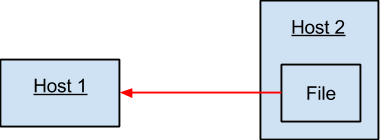
\includegraphics[width=0.4\textwidth]{img/basic_transfer_example.png}
	\caption{Host 1 copying a file.
	         \label{fig:copy_example}}
\end{figure}
For each transfer, a copy will be initiated from Host 1. A file from Host 2 will then be transferred to Host 1 using the particular protocol (see figure \ref{fig:copy_example}).

The tests will be run with 3 files: A 6 byte file containing the word `hello', a 350MB video file and a 1GB video file. The formats of these files were not tailored to the specific domain of bioinformatics because all 4 protocols are agnostic of format, and treat everything as binary.

\begin{figure}[H]
	\centering
	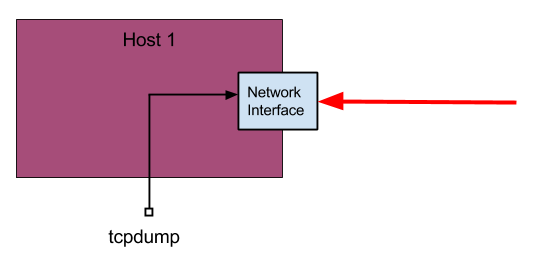
\includegraphics[width=0.5\textwidth]{img/if_example.png}
	\caption{The network interface capturing traffic.
             \label{fig:interface_example}}
\end{figure}
The `tcpdump' program (\url{www.tcpdump.org}) comes with most Unix systems. As depicted in figure \ref{fig:interface_example}, it watches a network interface (e.g.\ eth0) and logs information about packets which pass through. The program is run while each transfer is in progress, and the output is filtered to include only packets sent between Host 1 and Host 2. This output is used as the raw data for analysis.

This approach allows analysis of overhead (because \textit{all} transferred data is logged, rather than just the file size), speed (data/time), consistency, total time, and total size.

Note that despite the name, tcpdump can also capture UDP packets, which is relevant for some of the protocols.

\subsection{Implementation of Testbed}
A simple Python script will be sufficient to run the transfers, as most of the work will be done by a subprocess for each specific protocol. The analysis will also be done using Python as there are a vast number of analytical and visualisation tools available.

All testing will be done on an Ubuntu 14.04 system, with the following packages installed
\begin{itemize}
	\item python 2.7
	\item globus-gass-copy-progs 8.6
	\item globus-gridftp-server-progs 6.38
	\item tcpdump
	\item openssh-client
	\item openssh-server
	\item openssh-portable with the HPN patches, compiled from \url{https://github.com/rapier1/openssh-portable}
\end{itemize}
The testbed should work on any Unix system as long as Python, tcpdump and the binaries for each protocol are installed correctly.

The Python script for running the file transfers has been written to accept: The name of the network interface, the remote hostname (Host 2), the path of the file on Host 2, and a local path to copy the file to.
It then resolves the IPs of each host, and for each protocol, runs a transfer in isolation. 
\begin{figure}[H]
	\centering
	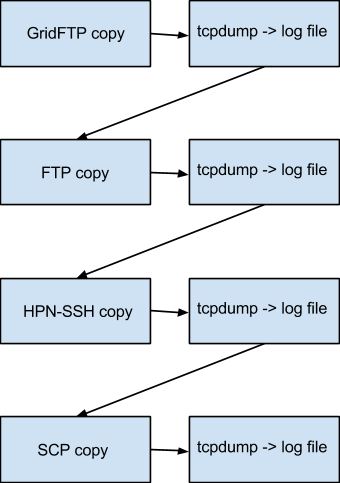
\includegraphics[height=0.5\textheight]{img/seq_example}
	\caption{The sequence of subprocesses called by the testbed.
	         \label{fig:testbed_sequence}}
\end{figure}
As seen in figure \ref{fig:testbed_sequence}, it spawns a tcpdump subprocess, and lets it run for precisely as long as the copy runs. The tcpdump program is started with filters, so that only traffic between the two hosts is captured. It then saves the output in a file.

This allows for a much more controlled environment, because the tcpdump only captures while the copy is running, no other packets will be included in the logs. Also, the copies are run programmatically and consecutively. Successive copies are not started until both the tcpdump and protocol processes have been closed, and the log file has been written. This means that they are all run in an identical (within reason) environment, but at the same time do not interfere with each other.

This test process is run multiple times for statistical reasons, generating multiple log files.

A separate Python file then reads in the log files and parses them. This information is used to calculate metrics and display graphs.
Operations can then be run by looking at the time of each packet, and the size of its payload. 

This data can then be aggregated over multiple log files, and graphed using the matplotlib Python library.

\section{Results}
Please note that the following data was not collected from the final tests. It represents a test run between my lab machine at UCT, and my DigitalOcean VM in a datacenter in Amsterdam. The environment was not controlled, and the connection was absolutely \textit{not} stable. In fact, you will be able to see this from the graph depicting individual packets. This section will be replaced with real data, and just serves to demonstrate the \textit{kinds} of graphs that can be included. 

\begin{figure*}
	\centering
	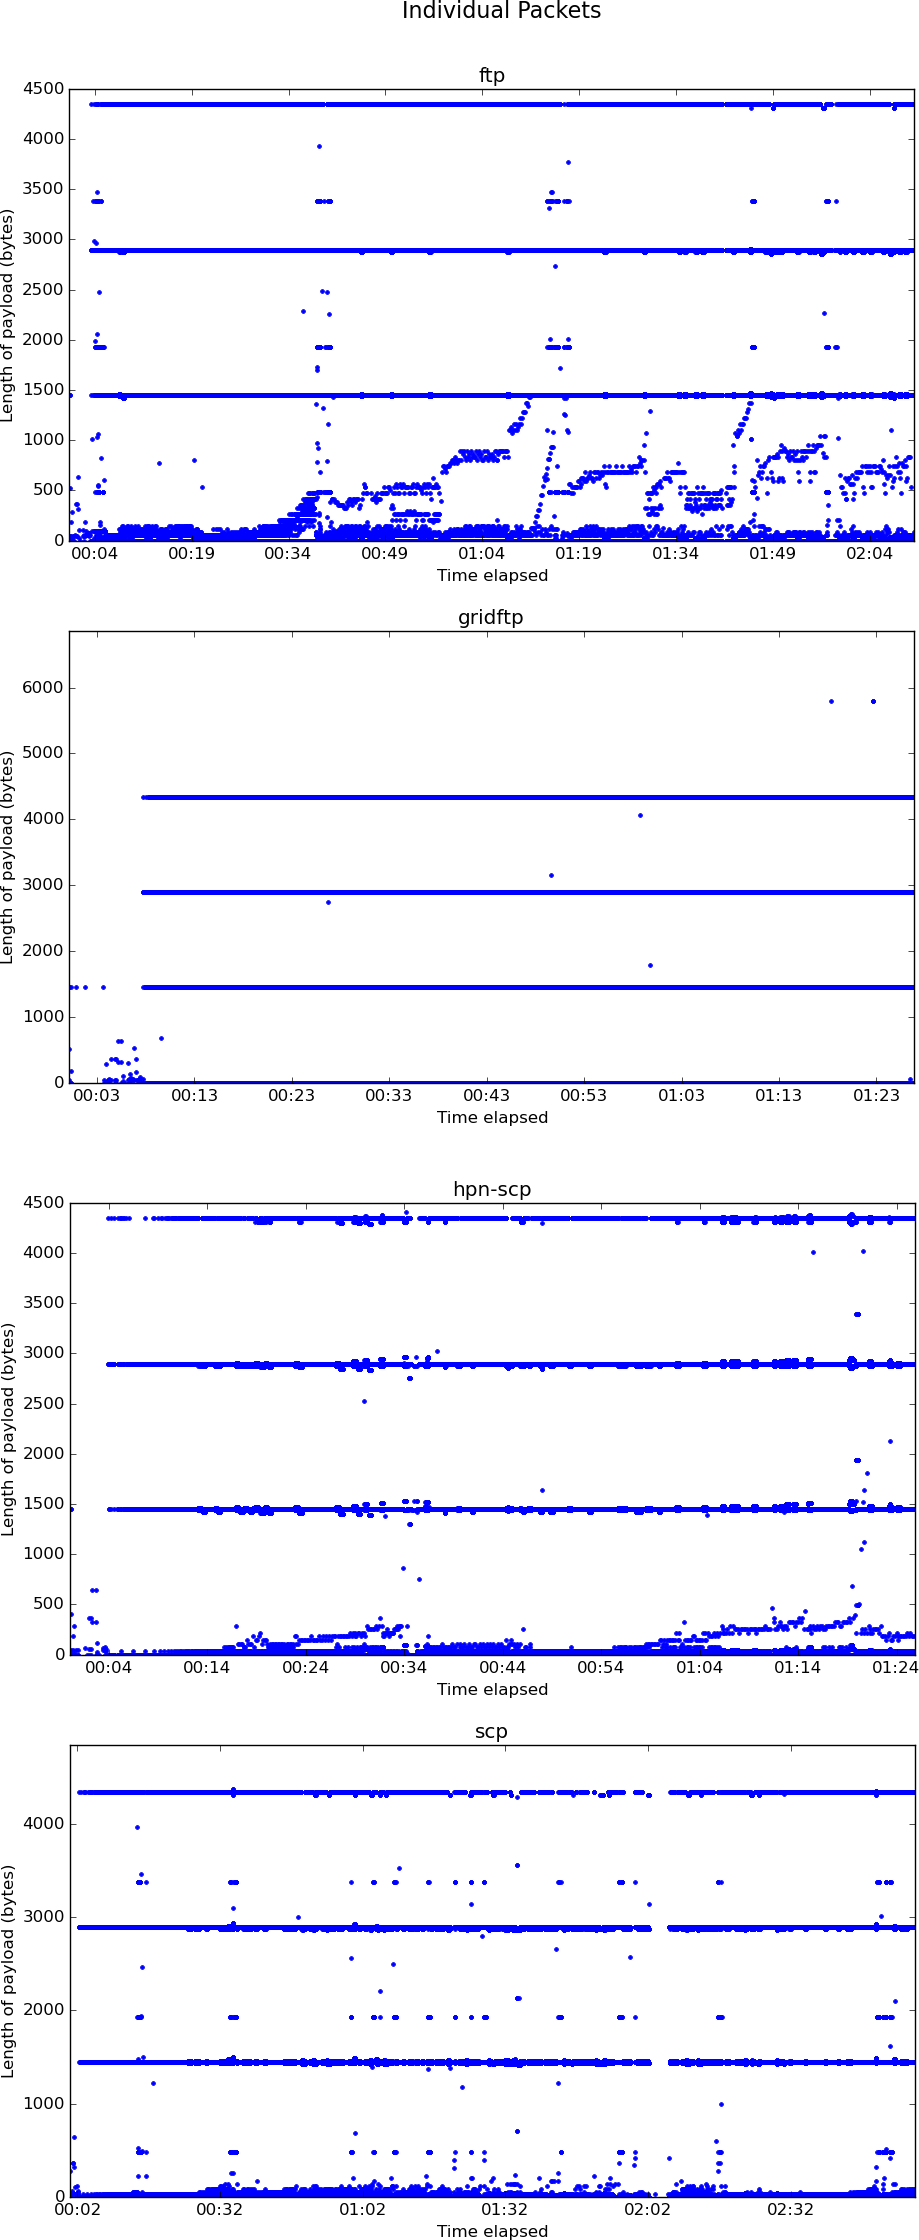
\includegraphics[height=\textheight]{img/testdata_packets.png}
	\caption{A graphical representation of each transfer
	         \label{fig:testdata_packets}}
\end{figure*}
Figure \ref{fig:testdata_packets} shows each packet of the transfer as a dot, where the x axis is time and the y axis shows the payload length in bytes.

\begin{figure*}
	\centering
	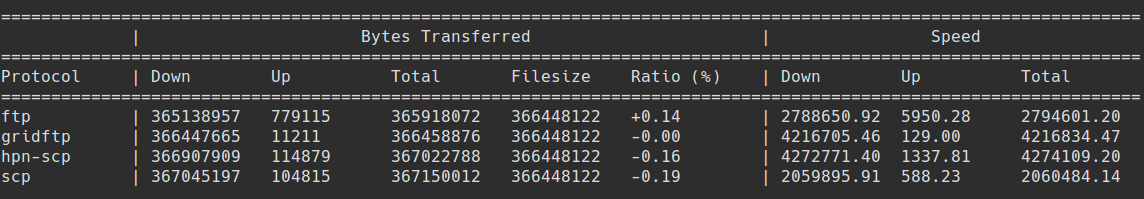
\includegraphics[width=\textwidth]{img/testdata_detail.png}
	\caption{The raw data, aggregated per protocol
	         \label{fig:testdata_detail}}
\end{figure*}
Figure \ref{fig:testdata_detail} is what the analysis suite outputs if no arguments for graphs are specified. It is representing the same data, but shows it in a way which is easier to see actual values.

\begin{figure*}
	\centering
	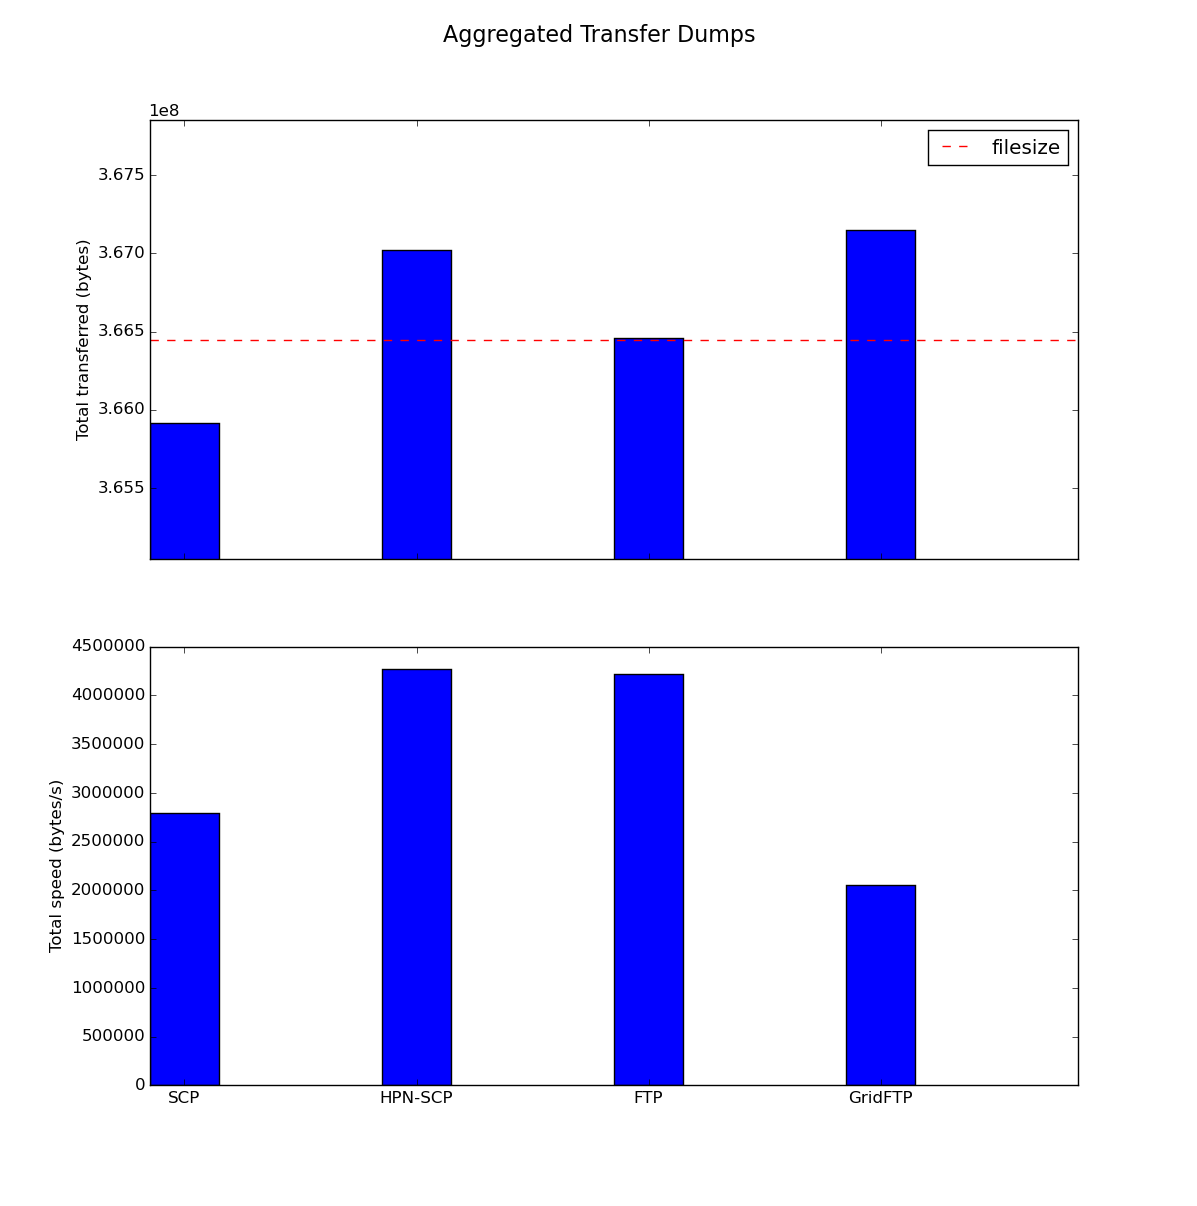
\includegraphics[width=\textwidth]{img/testdata_aggregate.png}
	\caption{Aggregated data per protocol, with a line representing filesize
	         \label{fig:testdata_aggregate}}
\end{figure*}

Figure \ref{fig:testdata_aggregate} shows the same data as figure \ref{fig:testdata_detail}, but displayed as a bar graph. This facilitates easier comparison between protocols, and makes it easy to see how much overhead (or compression) was used by comparing the bars to the filesize line.

\section{Acknowledgements}
TODO

\bibliographystyle{ACM-Reference-Format-Journals}
\bibliography{ref} 


\end{document}

